% Condensed subsections for inclusion in the main paper.
% Requires: amsmath, amssymb, booktabs, longtable
%
% Cross-references to the validated linear algebra section (sec:validated-linalg):
%   thm:schur-to-resolvent-generic, prop:triangular-circle,
%   lem:block-weyl, lem:schur-defect-to-E, lem:proj-triangle-split,
%   lem:proj-controls-eval, eq:proj-bound-schur, eq:proj-bound-ord,
%   subsec:contour-suprema, subsec:proj-split-schur-ord
%
% Cross-references to supplementary material (supplementary_material.tex):
%   S-tab:two-stage-results, S-tab:resolvent-bounds,
%   S-tab:spectral-coefficients, S-tab:tail-bounds-sample,
%   S-thm:two-stage
%
% xr is set up in Gauss.tex (xr-hyper + \externaldocument).
% Compile supplementary_material.tex first to generate its .aux file.

% =====================================================================
\subsection{Certified resolvent bounds on contours}
\label{sec:certified-resolvent}

To lift the finite-dimensional spectral data of $L_K$ to the
infinite-dimensional operator $L : H^2(D_1) \to H^2(D_1)$,
we verify the \emph{small-gain condition}: for each eigenvalue
$\lambda_j$ and an excluding circle
$\Gamma_j = \{z : |z - \hat\lambda_j| = r_j\}$,
\begin{equation}
\label{eq:small-gain}
\alpha_j \;=\; \varepsilon_K \cdot
  \sup_{z \in \Gamma_j} \|(z I - L_K)^{-1}\| \;< \;1,
\end{equation}
where $\varepsilon_K = C_2 (2/3)^{K+1}$ is the truncation error bound
(Theorem~\ref{thm:one-sided-approxs}).
When \eqref{eq:small-gain} holds, $\Gamma_j \subset \rho(L)$ and $L$
has exactly as many eigenvalues (counted with multiplicity) inside
$\Gamma_j$ as $L_K$.

We employ a \emph{two-stage} strategy, following the
certification workflow of \S\ref{subsec:contour-suprema}.
For eigenvalues $j = 1, \ldots, 15$, the resolvent of the full matrix
$L_{48}$ is sampled at $256$ points on $\Gamma_j$ and certified
via Theorem~\ref{thm:schur-to-resolvent-generic}
(Schur defects $\to$ resolvent bound),
yielding $\alpha_j \leq 6.2 \times 10^{-1}$
($\varepsilon_{48} \approx 2.37 \times 10^{-8}$).
For $j = 16, \ldots, 50$, the eigenvalue gaps shrink below $10^{-7}$
and the resolvent of $L_{48}$ becomes too large;
instead, we certify the resolvent at $K = 256$
($\varepsilon_{256} \approx 5.59 \times 10^{-45}$)
using the \emph{block Schur method}: the certified Schur form
$L_{256} = Q T Q^*$ is partitioned around $\lambda_j$
(Lemma~\ref{lem:block-weyl}), and the
resolvent supremum on each circle $\Gamma_j$ is certified by
Proposition~\ref{prop:triangular-circle},
giving $\alpha_j \leq 3.14 \times 10^{-4}$
for all $50$ eigenvalues.

The certified finite-dimensional resolvent $\|R_{L_K}\|$ is then
lifted to the infinite-dimensional one via Neumann perturbation:
\[
\|R_L(z)\| \;\leq\; \frac{\|R_{L_K}(z)\|}{1 - \alpha_j}
\;=:\; M_{\infty,j}.
\]
The full results are given in the supplementary material
(Tables~\ref{S-tab:two-stage-results} and~\ref{S-tab:resolvent-bounds}).
All $50$ excluding circles are certified, proving that the first $50$
eigenvalues of~$L$ are simple.

% =====================================================================
\subsection{Eigenvalue, eigenvector, and projector enclosures}
\label{sec:enclosures}

The resolvent certification also yields bounds on the Riesz projector errors.
Writing $P_j = P_L(\Gamma_j)$ and $P_{K,j} = P_{L_K}(\Gamma_j)$
for the spectral projectors of $L$ and $L_K$ associated with
the excluding circle $\Gamma_j$, the contour integral representation gives
\begin{equation}
\label{eq:proj-error}
\vartheta_j \;:=\; \|P_j - P_{K,j}\|
\;\leq\; \frac{|\Gamma_j|}{2\pi} \cdot
  \frac{M_{\infty,j}^2 \cdot \varepsilon_K}{1 - \alpha_j}.
\end{equation}
At the \emph{finite-dimensional level}, the projector error
$\|P_{L_K}(\Gamma_j) - \tilde P_T(\Gamma_j)\|$ arising from the
numerical Schur decomposition and reordering is bounded by the
decomposition of Lemma~\ref{lem:proj-triangle-split}: the Schur
residual contributes~\eqref{eq:proj-bound-schur} and the ordschur
reordering contributes~\eqref{eq:proj-bound-ord}.
At $K = 256$, $\vartheta_j$ ranges from $1.01 \times 10^{-41}$ ($j = 1$)
to $2.96 \times 10^{-3}$ ($j = 35$).  For $j \geq 36$, useful
projector bounds require $K = 512$
(see supplementary Table~\ref{S-tab:two-stage-results}).

Since each $\lambda_j$ is certified simple and $\vartheta_j < 1$,
Lemma~\ref{lem:proj-controls-eval} gives the eigenvalue error bound
\begin{equation}
\label{eq:eval-from-proj}
|\lambda_j - \hat\lambda_j|
\;\leq\;
\frac{\varepsilon_K(1 + \vartheta_j) + 2C\,\vartheta_j}{1 - \vartheta_j},
\end{equation}
where $C = \|L_K\|$ is a certified upper bound on the
discretization norm and $\varepsilon_K = \|L - L_K\|$.
This avoids any Newton--Kantorovich argument: the projector error
\emph{alone} controls the eigenvalue error for all $50$ eigenvalues
simultaneously, with no requirement on the eigenvalue gap relative
to $\varepsilon_K$.  For the dominant eigenvalues ($j \leq 15$) the
bound~\eqref{eq:eval-from-proj} is of order $\varepsilon_K \sim 10^{-8}$
(at $K = 48$); for $j \leq 35$ at $K = 256$ it reaches $\sim 10^{-45}$.
The tightest enclosures use $K = 1024$ (2048-bit precision,
$\varepsilon_{1024} \approx 3.23 \times 10^{-180}$): for the leading
eigenvalues ($j \leq 15$) the enclosure radii are of
order $10^{-176}$--$10^{-171}$, degrading to $\sim 10^{-119}$ for
$j = 50$ due to resolvent growth on the excluding circles.
In particular, $\lambda_2^* \in B(-0.303663002899, \; 5 \times 10^{-176})$,
certifying the Wirsing constant to over $175$ decimal digits.
The full list of eigenvalue enclosures is given in the supplementary
material (Table~\ref{S-tab:two-stage-results}).

The eigenvectors $\hat v_j$
of $L_K$ are the first columns of the ordered Schur unitary $Q_{\mathrm{ord}}$,
known to within the combined Schur and ordschur similarity defect
$\|E\| \leq 5.72 \times 10^{-317}$ at $K = 1024$
(supplementary Table~\ref{S-tab:spectral-data-K1024}).
At the \emph{infinite-dimensional level}, the projector error
$\vartheta_j$ controls the gap between the true eigenvector $v_j$ of
$L$ and $\hat v_j$ of $L_K$:
$\|v_j - \hat v_j\| \leq 2\vartheta_j / (1 - \vartheta_j)$.

Since $L$ is non-normal, the spectral expansion requires the dual eigenvectors
$\ell_j$.  We compute the spectral coefficient
$\ell_j(\mathbf{1}) = e_1^* P_j e_1$ from the ordered Schur form:
with $T_{\mathrm{ord}} =
  \bigl[\begin{smallmatrix} \lambda_j & T_{12} \\ 0 & T_{22}\end{smallmatrix}\bigr]$
and $q = Q_{\mathrm{ord}}^* e_1$,
\begin{equation}
\label{eq:ell-formula}
\ell_j(\mathbf{1})
  = q_1 - T_{12} \cdot (T_{22} - \lambda_j I)^{-1} q_{\mathrm{rest}},
\end{equation}
where the triangular system is solved in $P$-bit BigFloat arithmetic.
The certified error is dominated by the Schur similarity defect
$\|E\| \leq r_{\mathrm{sch}}\sqrt{1+\delta} + C_A\,\delta$
(Lemma~\ref{lem:schur-defect-to-E}); the triangular solve
residual is negligible ($\sim 10^{-617}$ at 2048-bit).

At $K = 1024$ (2048-bit precision, $\|E\| \leq 5.72 \times 10^{-317}$),
all $50$ spectral coefficients are \emph{sign-certified}:
$|\ell_j(\mathbf{1})| > \delta_j$ with radii
$\delta_j \in [4.5 \times 10^{-316},\; 1.1 \times 10^{-282}]$.
The signs alternate as
$\ell_1 > 0$, $\ell_2 > 0$, $\ell_3 < 0$, $\ell_4 > 0$, \ldots,
with $|\ell_j(\mathbf{1})| \sim |\lambda_j|$ for large~$j$.
Cross-validation at $K = 256$, $512$, and $1024$ confirms agreement
of all certified digits
(see supplementary Table~\ref{S-tab:spectral-data-K1024}).

% =====================================================================
\subsection{Certified spectral expansion and computation of $F_n(x)$}
\label{sec:spectral-expansion}

With all $50$ eigenvalues certified simple and the spectral
coefficients $\ell_j(\mathbf{1})$ sign-certified, the spectral
expansion
\begin{equation}
\label{eq:spectral-exp-main}
L^n \mathbf{1}
  = \sum_{j=1}^{N} \lambda_j^n \, \ell_j(\mathbf{1}) \, v_j + R_N(n)
\end{equation}
holds rigorously in $H^2(D_1)$ with the tail bound
\begin{equation}
\label{eq:tail-bound}
\|R_N(n)\| \;\leq\; \rho^{n+1} \cdot M_\infty \cdot \|Q_N \mathbf{1}\|,
\end{equation}
where $Q_N = I - \sum_{j=1}^{N} P_j$ is the tail projector,
$\rho$ is the radius of a separating circle in the eigenvalue gap
$|\lambda_{N+1}| < \rho < |\lambda_N|$, and $M_\infty$ is the certified
resolvent on this circle.  For $N = 50$, the parameters are
$\rho = 1.014 \times 10^{-21}$,
$M_\infty = 6.062 \times 10^{41}$,
and $\|Q_{50}\mathbf{1}\| \leq 6.138 \times 10^{-21}$
(computed at $K = 512$), giving
$\|R_{50}(n)\| \leq 3.72 \times 10^{21} \cdot (1.01 \times 10^{-21})^{n+1}$.
Already at $n = 1$ the remainder is below $10^{-20}$; at $n = 5$ it drops
below $10^{-104}$ (see supplementary Table~\ref{S-tab:tail-bounds-sample}).

Define the integrated spectral expansion
\[
F_n^{(j_0)}(x) \;=\; \int_0^x
  \sum_{j=j_0}^{N} \lambda_j^n \,\ell_j(\mathbf{1})\, v_j(t)\, dt,
\]
which is computed exactly in the shifted monomial basis via
$\int_0^x (t-1)^k\,dt = \bigl((x{-}1)^{k+1} - (-1)^{k+1}\bigr)/(k{+}1)$.
For $j_0 = 2$, this measures the integrated deviation of $L^n\mathbf{1}$
from its equilibrium $\ell_1(\mathbf{1})\,v_1$.  The $L^\infty$ error
is controlled by Cauchy--Schwarz and the Gram matrix of the basis on
$[0,1]$ (spectral norm $\leq \pi$):
\[
\sup_{x \in [0,1]} \Bigl|F_n^{(j_0)}(x) - \int_0^x \!\Bigl(L^n\mathbf{1}
  - \textstyle\sum_{j<j_0} \lambda_j^n P_j\mathbf{1}\Bigr) dt \Bigr|
\;\leq\; \sqrt{\pi}\;\rho^{n+1} \cdot C
\;\leq\; 6.6 \times 10^{21} \cdot (1.01 \times 10^{-21})^{n+1}.
\]
Figure~\ref{fig:integrated-spectral} shows $F_n^{(j_0)}$ for
$j_0 = 2, \ldots, 6$ and $n = 1, 2, 5$.  As dominant eigenfunctions are
progressively removed, the Markov partition structure of the Gauss map
becomes increasingly visible, and the amplitude decreases by roughly a
factor $|\lambda_{j_0}/\lambda_{j_0-1}| \approx 1/3$ per removed mode.

\begin{figure}[htbp!]
\centering
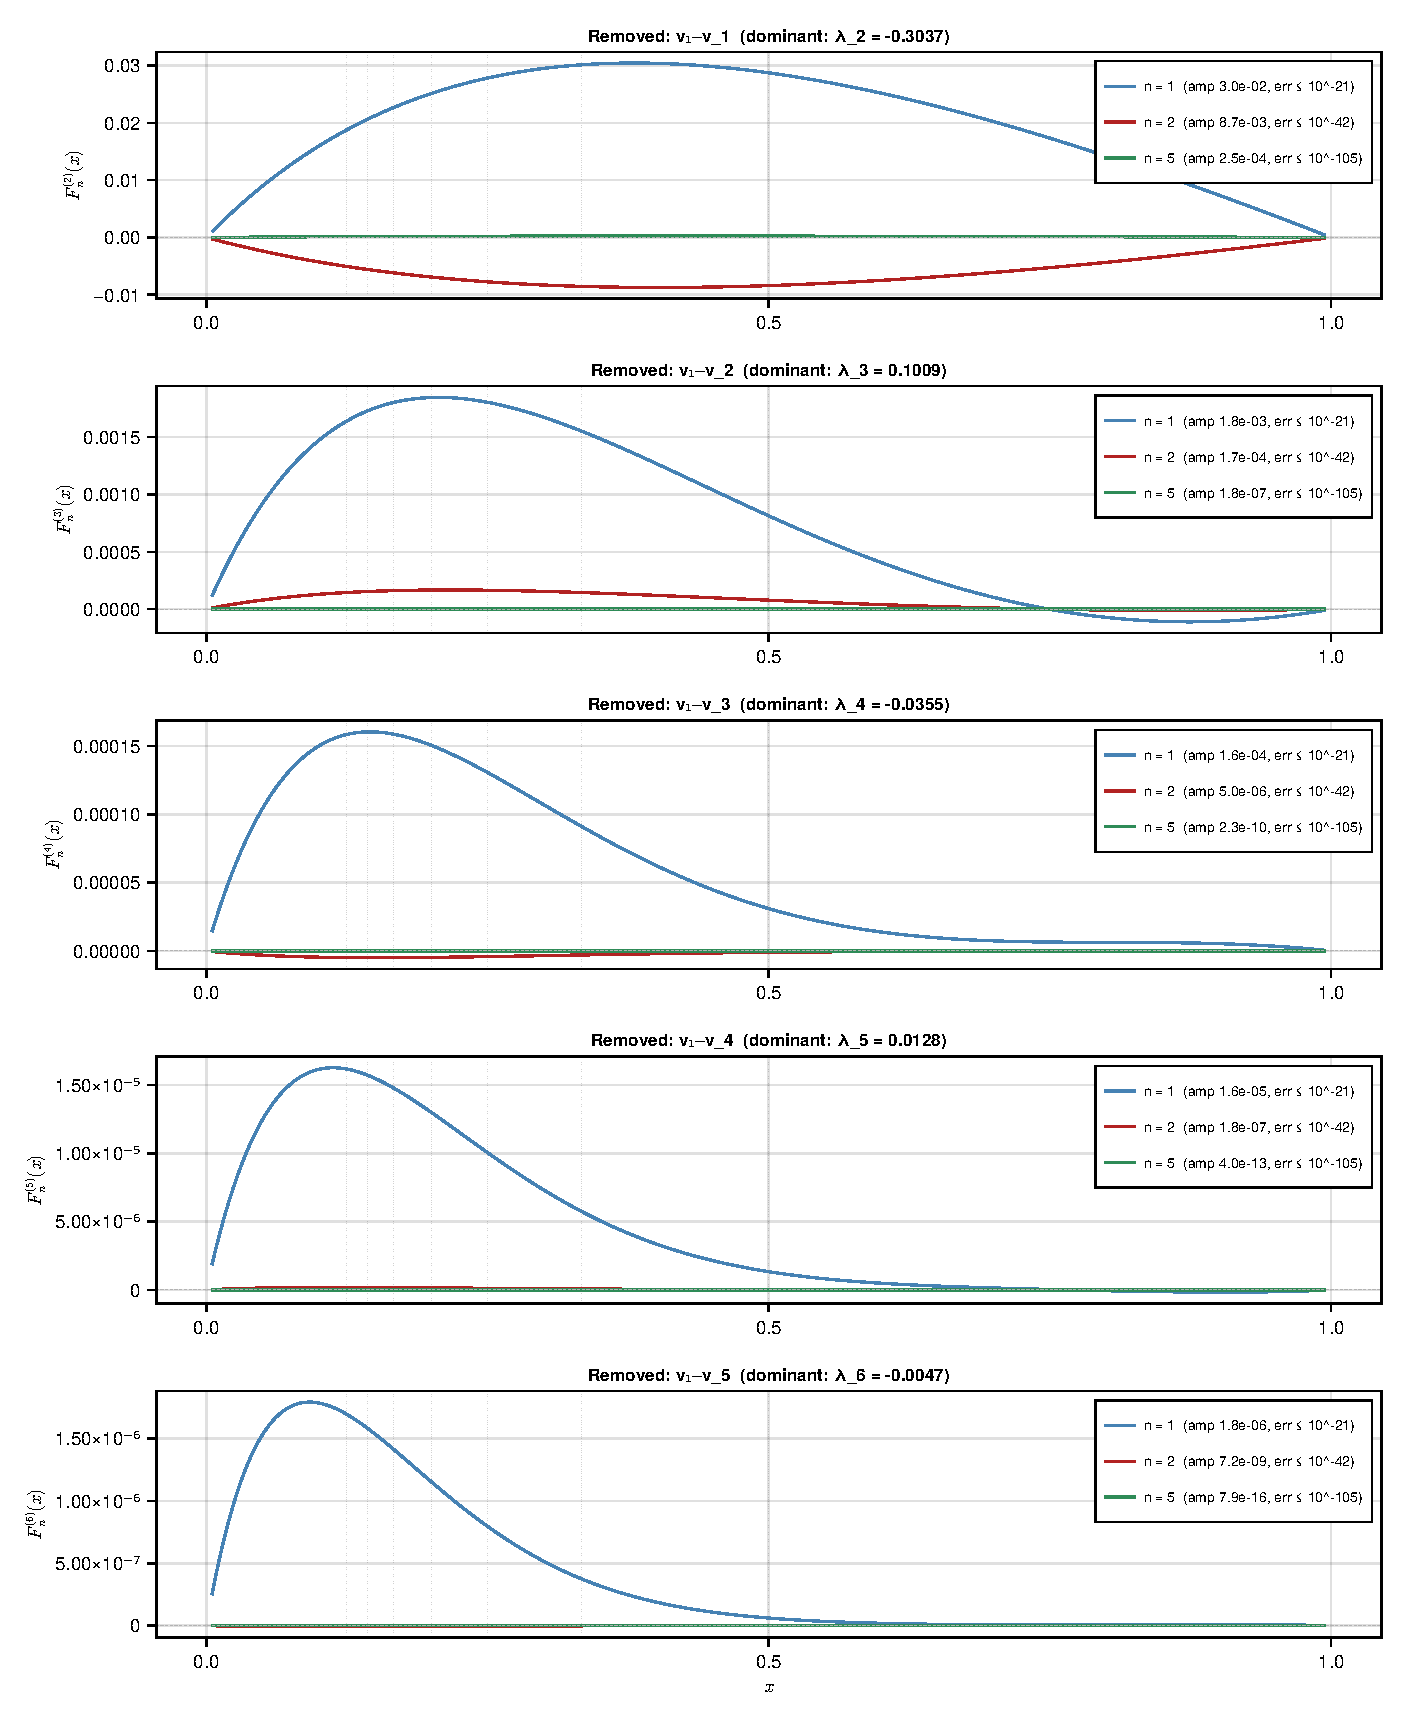
\includegraphics[width=0.75\textwidth]{integrated_spectral_progressive.pdf}
\caption{Integrated spectral expansion
$F_n^{(j_0)}(x) = \int_0^x \sum_{j \geq j_0}
  \lambda_j^n\,\ell_j(\mathbf{1})\,v_j(t)\,dt$
with the first $j_0 - 1$ eigenfunctions cumulatively removed.
Each panel shows $n = 1$ (blue), $n = 2$ (red), $n = 5$ (green).
Dotted vertical lines mark the Markov partition boundaries $x = 1/k$.
For $j_0 = 6$, $n = 5$, the signal amplitude is ${\sim}\,10^{-16}$
while the $L^\infty$ error bound is ${\leq}\,10^{-105}$, confirming
that the plotted curves are rigorous to plotting accuracy.}
\label{fig:integrated-spectral}
\end{figure}

Returning to the Gauss--Kuzmin problem, the distribution function
$G_n(x) = \int_0^x L^n\mathbf{1}(t)\,dt$ converges to $\log_2(1+x)$.  Since $\lambda_1 = 1$ and
$\ell_1(\mathbf{1})\,v_1 = \frac{1}{\ln 2} \cdot \frac{1}{1+x}$
(the invariant density), the spectral expansion gives
\[
|G_n(x) - \log_2(1{+}x)|
\;\leq\; |F_n^{(2)}(x)| + \sqrt{\pi}\;\|R_N(n)\|.
\]
The dominant error term is $\lambda_2^n\,\ell_2(\mathbf{1})\,\int_0^x v_2$,
which decays at rate $|\lambda_2|^n \approx 0.3037^n$, the
Wirsing constant.  The tail bound certifies that the
$50$-term expansion captures this rate with
rigorous error below $10^{-20}$ already at $n = 1$.
Figure~\ref{fig:spectral-convergence} illustrates the convergence:
the spectral approximant $S_{50}(n,x)/\lambda_1^n$ rapidly approaches
the invariant density $\ell_1(\mathbf{1})\,v_1(x)$, with the spectral
gap $|\lambda_2/\lambda_1| \approx 0.304$ governing the rate.

\begin{figure}[htbp!]
\centering
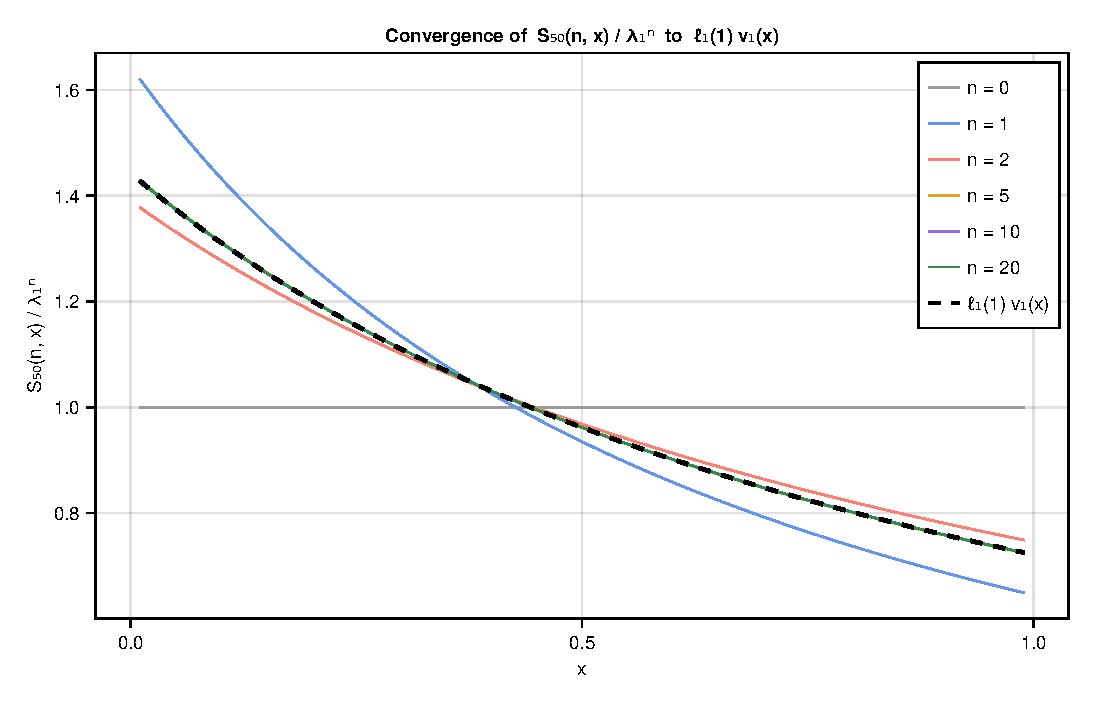
\includegraphics[width=0.65\textwidth]{spectral_convergence.pdf}
\caption{Convergence of the spectral approximant
$S_{50}(n,x) = \sum_{j=1}^{50} \lambda_j^n\,\ell_j(\mathbf{1})\,v_j(x)$
(normalized by $\lambda_1^n$) to the invariant density
$\ell_1(\mathbf{1})\,v_1(x) = \frac{1}{\ln 2(1+x)}$ (dashed black).
The spectral gap $|\lambda_2/\lambda_1| \approx 0.304$ governs the
convergence rate: by $n = 5$ the approximation is indistinguishable
from the limit.}
\label{fig:spectral-convergence}
\end{figure}
